Em contextos nos quais há uma demanda por software que precisa ser rapidamente atendida ou quando os requisitos mudam rapidamente, processos de desenvolvimento ágil são recomendados. Estes processos possuem natureza iterativa, nos quais as fases de especificação, projeto, desenvolvimento e teste se intercalam. Como consequência, o software é entregue não em uma versão final acabada, mas em uma série de incrementos de novas funcionalidades.
\cite{Sommerville:Livro}.

Na década de 1990, houve uma demanda ainda maior para que os esforços das equipes de desenvolvimento se concentrassem no software somente, diminuindo o ônus em projeto e documentação. Em resposta, foi proposto o  ``Manifesto para o Desenvolvimento Ágil'' (\textit{The Manifesto for Agile Software Development}) \cite{KentBeck:ManifestoAgil}, no qual foi proposta a abordagem iterativa para especificação, desenvolvimento e entrega do software para cenários com requisitos que mudam rapidamente e nos quais se deseja entregar um software rapidamente ao cliente. O Manifesto para o Desenvolvimento Ágil possui quatro valores, são eles:

\begin{enumerate}
	\item Indivíduos e interações acima de processos e ferramentas;
	\item Software operacional acima de documentação completa;
	\item Colaboração dos clientes acima de negociação contratual;
	\item Respostas a mudanças acima de seguir um plano \cite{Pressman:Livro}.
\end{enumerate}

Os princípios do Manifesto Ágil consideram como prioridade a satisfação do cliente e o acolhimento dos pedidos de alterações. A medida de progresso considerada é a entrega de software em funcionamento ao cliente, razão pela qual há várias entregas do software desenvolvido em intervalos pequenos de tempo. Ressalta-se a importância da motivação da equipe engajada no projeto, que deve trabalhar em conjunto diariamente, com uma comunicação fluida e, preferencialmente, presencial. A simplicidade, auto-organização e avaliação em intervalos regulares complementam esses princípios \cite{KentBeck:ManifestoAgil}.

Atualmente, existe um vasto número de modelos de processo ágeis que satisfazem aos princípios do Manifesto Ágil, inclusive com muitas semelhanças filosóficas e práticas entre eles. Exemplos de modelos de processos ágeis são: SCRUM, \emph{eXtreme Programming}, \emph{Feature Driven Development}, \emph{Agile Unified Process}, dentre outros.

O \emph{Processo Unificado Ágil} (AUP - \textit{Agile Unified Process}), em particular, é um modelo ágil para o desenvolvimento de software. O AUP é baseado em um processo de desenvolvimento de software clássico, o RUP (\textit{Rational Unified Process}). O RUP é destinado a grandes projetos que envolvam um grande número de pessoas em sua equipe de desenvolvimento. Ao conceber o AUP, o seu criador, Scott Ambler, procurou adaptar as boas práticas do RUP a pequenos projetos. Através de uma metodologia simples e de fácil compreensão, usando técnicas e conceitos ágeis para o desenvolvimento de software, o AUP segue uma filosofia ágil permanecendo fiel às práticas do RUP \cite{Ambler:Livro}.


O AUP possui quatro fases de desenvolvimento, são elas:

\begin{itemize}
	\item \textbf{Concepção (\textit{Inception}).} O objetivo é identificar o escopo inicial do projeto e a arquitetura potencial do sistema a fim de gerar estimativas financeiras e prover informações que subsidiem a aceitação pelas partes interessadas;
	\item \textbf{Elaboração (\textit{Elaboration}).} O objetivo é prover uma arquitetura central, resolução dos altos riscos e definição de estimativas mais realistas;
	\item \textbf{Construção (\textit{Construction}).} O objetivo é construir o software, trabalhando em uma base incremental regular, que atende às necessidades de maior prioridade das partes interessadas no projeto;
	\item \textbf{Transição (\textit{Transition}).} O objetivo é validar e implantar o sistema em seu ambiente de produção.
\end{itemize}

As fases do AUP não são realizadas em cascata. Ao contrário, há diversas iterações e podem existir atividades de fases distintas sendo executadas em paralelo. Uma ideia do ciclo de vida do AUP que ilustra esta característica pode ser visualizada na Figura \ref{fig:aupciclo}.

\begin{figure}[H]
	\centering
	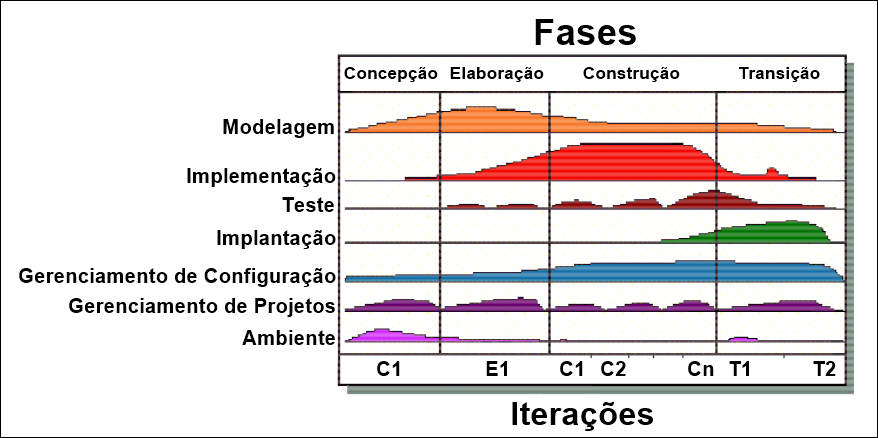
\includegraphics[scale=0.7]{./img/aupOficial.png}
	\caption{Ciclo de vida do AUP.} \label{fig:aupciclo}
\end{figure}

Ainda conforme a Figura \ref{fig:aupciclo}, é possível identificar as sete disciplinas que compõem o AUP. Elas definem um conjunto de atividades (e artefatos relacionados) que são realizados ao longo das iterações de desenvolvimento. Estas disciplinas são definidas como segue:

\begin{itemize}
	\item \textbf{Modelagem (\textit{Model})}. O objetivo desta disciplina é promover o entendimento do negócio da organização, o domínio do problema a ser abordado pelo projeto, e a identificação de uma solução viável para resolver o domínio do problema;
	\item \textbf{Implementação (\textit{Implementation})}. O objetivo desta disciplina é o de transformar o(s) modelo(s) em código executável e executar um nível básico de testes, nomeadamente os testes de unidades;
	\item \textbf{Teste (\textit{Test})}. O objetivo desta disciplina é a realização de uma avaliação objetiva para garantir a qualidade. Isto inclui as atividades de validação e verificação dos requisitos;
	\item \textbf{Implantação (Deployment)}. O objetivo desta disciplina é planejar a entrega do sistema e executar este plano a fim de tornar o sistema disponível para os usuários finais;
	\item \textbf{Gerenciamento de Configuração (\textit{Configuration Management})}. O objetivo desta disciplina é o de gerir o acesso aos artefatos criados durante todas as fases do desenvolvimento do software. Isso inclui não apenas controlar versões de artefatos ao longo do tempo, mas também controlar e gerenciar mudanças;
	\item \textbf{Gerenciamento de Projetos (\textit{Project Management})}. O objetivo desta disciplina é a de dirigir as atividades que ocorrem no projeto. Isto incluir a gestão de riscos, a coordenação de pessoas e controle de prazos e orçamento;
	\item \textbf{Ambiente (\textit{Environment})}. O objetivo desta disciplina é o de apoiar o resto do esforço, garantido que o processo adequado, orientação (normas e diretrizes) e ferramentas (hardware, software, etc) estejam disponíveis para a equipe quando necessário \cite{Ambler:Livro}.
\end{itemize}

Durante uma iteração, o trabalho prossegue na maioria ou em todas as disciplinas. Entretanto, o esforço relativo no decorrer destas disciplinas muda ao longo do tempo. As iterações iniciais tendem a dar uma ênfase maior aos requisitos e ao projeto, enquanto que as últimas disciplinas dão a esses itens uma ênfase menor, à medida que os requisitos e o projeto central se estabilizam por meio de um processo de realimentação e adaptação \cite{Larman:Livro}.
